\section{Results}
\label{sec:results}

All intervals are 95\% cluster-bootstrap intervals; ``BAcc'' is balanced accuracy at the threshold $\tau^\mathrm{bal}$ fitted on the calibration split of the same domain unless stated otherwise.

\subsection{Natural data (RQ1)}
\label{sec:res-natural}

\begin{table*}[t]
\centering\small
\setlength{\tabcolsep}{3.2pt}
\resizebox{\textwidth}{!}{\begin{tabular}{lrrrrrrrrrrrl}
\toprule
 & \multicolumn{2}{c}{RT-QA} & \multicolumn{2}{c}{RT-Sum} & \multicolumn{2}{c}{RT-D2T} & \multicolumn{2}{c}{FaithBench} & \multicolumn{2}{c}{HaluEval-QA} & \multicolumn{2}{c}{RAGTruth pooled} \\
Method & AUC & BAcc & AUC & BAcc & AUC & BAcc & AUC & BAcc & AUC & BAcc & BAcc & 95\% CI \\
\midrule
Token precision & .723 & .640 & .676 & .616 & .692 & .632 & .619 & .592 & .898 & .916 & .586 & [.564, .607] \\
TF--IDF cosine & .620 & .582 & .667 & \textbf{.638} & .671 & .620 & .617 & \textbf{.601} & .364 & .500 & .640 & [.621, .659] \\
\midrule
MiniLM cosine (document) & .523 & .521 & .593 & .540 & .541 & .536 & .576 & .536 & .237 & .500 & .551 & [.526, .577] \\
MiniLM cosine (mean-max) & .683 & .626 & .620 & .597 & .645 & .604 & .513 & .513 & .251 & .498 & .611 & [.592, .630] \\
MiniLM cosine (min-max) & .679 & .647 & .581 & .564 & .565 & .559 & .505 & .510 & .255 & .498 & .535 & [.515, .554] \\
BGE-small cosine (mean-max) & .689 & .643 & .648 & .614 & .698 & .637 & .522 & .498 & .247 & .500 & .591 & [.572, .611] \\
\midrule
BERTScore & .723 & .649 & .619 & .585 & .617 & .580 & .569 & .525 & .329 & .499 & .568 & [.547, .590] \\
NLI (SummaC-ZS style) & .654 & .630 & \textbf{.678} & .599 & .678 & \textbf{.642} & .546 & .544 & .747 & .748 & .613 & [.594, .633] \\
\midrule
Risk model: cosine only & .666 & .628 & .622 & .585 & .615 & .585 & .535 & .520 & .244 & .498 & .575 & [.553, .597] \\
Risk model: cosine + checks & .721 & .661 & .626 & .589 & .671 & .630 & .572 & .574 & .304 & .499 & \textbf{.673} & [.654, .691] \\
Risk model: full & \textbf{.808} & \textbf{.739} & .673 & .612 & \textbf{.703} & .635 & \textbf{.637} & .595 & \textbf{.977} & \textbf{.954} & .631 & [.609, .652] \\
\bottomrule
\end{tabular}
}
\caption{Evidence-grounded faithfulness on the full test splits. AUC treats \emph{unsupported} as the positive class; BAcc at the calibration-fitted $\tau^\mathrm{bal}$. ``RAGTruth pooled'' uses per-task thresholds and pools the \NTestRagtruth\ RAGTruth test examples. Bold: best per column. HaluEval-QA labels are synthetic.}
\label{tab:main}
\end{table*}

\paragraph{Faithfulness.} Table~\ref{tab:main} gives the cheap evaluators on the full test splits. No cheap method is good in absolute terms. On pooled RAGTruth, MiniLM mean-max cosine reaches a balanced accuracy of \PoolCosBacc\ \PoolCosBaccCi, the same as the NLI scorer (\PoolNliBacc\ \PoolNliBaccCi) and below plain TF--IDF cosine; BGE-small and BERTScore rank better than MiniLM (AUC \PoolBgeAuc\ and \PoolBertAuc\ vs.\ \PoolCosAuc) but do not threshold better. The sentence-level configuration matters more than the encoder: comparing the whole answer with the whole evidence (``document'') is the weakest embedding configuration on RAGTruth. The full risk model has the highest ranking quality (pooled AUC \PoolRiskAuc), but at its calibration-fitted threshold its pooled balanced accuracy (\PoolRiskBacc) is below that of the cosine-plus-checks variant (\PoolRiskChkBacc\ \PoolRiskChkBaccCi): its threshold carries a false-acceptance rate of \PoolRiskFar\% onto the test split, which already shows that a good ranking does not imply a good fixed threshold.

Two out-of-domain sets bracket these numbers. On FaithBench, which collects summaries that earlier detectors disagree on, every cheap method is close to chance (AUC \FbCosAuc\ for cosine, \FbNliAuc\ for NLI, at most \FbRiskAuc\ for the risk model). On HaluEval-QA every embedding method is \emph{below} chance (MiniLM AUC \HaluCosAuc\ \HaluCosAucCi): the synthetic hallucinated answers are on average \emph{more} similar to the knowledge passage than the correct ones. The risk model reaches AUC \HaluRiskAuc, but a model that sees only the three length features already reaches \AblOnlyLengthHaluAuc\ on HaluEval-QA (Table~\ref{tab:ablation}), so this number measures an artefact of how the benchmark was built, not grounding \citep{hussain2026parallax}.

\begin{table}[t]
\centering\small
\setlength{\tabcolsep}{3pt}
\resizebox{\columnwidth}{!}{\begin{tabular}{lrrlrr}
\toprule
Method & AUC & BAcc & 95\% CI & FAR & FRR \\
\midrule
Exact match & .582 & .582 & [.578, .585] & 0.2 & 83.5 \\
Reference containment & .880 & .880 & [.869, .889] & 3.4 & 20.7 \\
Token F1 & .874 & .811 & [.795, .828] & 32.4 & 5.4 \\
TF--IDF cosine & .825 & .793 & [.778, .807] & 16.0 & 25.4 \\
\midrule
MiniLM cosine (document) & .802 & .738 & [.722, .752] & 27.9 & 24.6 \\
MiniLM cosine (question+answer) & .813 & .738 & [.722, .754] & 29.8 & 22.6 \\
BGE-small cosine (document) & .835 & .759 & [.743, .775] & 30.6 & 17.5 \\
BERTScore & .737 & .687 & [.672, .702] & 29.9 & 32.7 \\
NLI (SummaC-ZS style) & .884 & .820 & [.807, .832] & 24.1 & 11.9 \\
\midrule
Risk model: cosine only & .837 & .756 & [.740, .770] & 24.5 & 24.3 \\
Risk model: full & \textbf{.957} & \textbf{.901} & [.889, .910] & 11.0 & 8.9 \\
\midrule
\multicolumn{6}{l}{\emph{Judged subset, $n=600$}} \\
Judge (3B) & .888 & .815 & [.777, .849] & 18.0 & 18.9 \\
Reference containment & .884 & .884 & [.859, .908] & 4.3 & 18.9 \\
MiniLM cosine (document) & .811 & .742 & [.699, .780] & 28.0 & 23.7 \\
Risk model: full & .959 & .917 & [.893, .942] & 8.1 & 8.4 \\
\midrule
\multicolumn{6}{l}{\emph{Judged subset, $n=150$}} \\
Judge (14B) & .957 & .881 & [.827, .924] & 2.9 & 20.9 \\
Reference containment & .903 & .903 & [.856, .946] & 2.9 & 16.5 \\
MiniLM cosine (document) & .810 & .742 & [.652, .821] & 22.9 & 28.7 \\
Risk model: full & .975 & .947 & [.903, .979] & 2.9 & 7.8 \\
\bottomrule
\end{tabular}
}
\caption{Reference-based correctness on EVOUNA-NQ (\NTestEvouna\ test answers). The lower block compares the small judge with cheap methods on the judged subset.}
\label{tab:evouna}
\end{table}

\paragraph{Correctness.} Against short reference answers (Table~\ref{tab:evouna}) lexical containment---does the answer contain a reference string---is a strong baseline (BAcc \EvContainBacc) and embedding cosine is clearly weaker (\EvCosBacc). NLI reaches \EvNliBacc. The ten-feature reference-mode risk model reaches \EvRiskBacc\ with a false-acceptance rate of \EvRiskFar\%. On the \EvJudgeSmallN\ judged answers, the small judge (\EvJudgeSmallBacc\ \EvJudgeSmallBaccCi) beats document cosine (cosine minus judge: \EvCosMinusSmall\ \EvCosMinusSmallCi) but loses to containment (containment minus judge: \EvContainMinusSmall\ \EvContainMinusSmallCi) and to the risk model (\EvRiskMinusSmall\ \EvRiskMinusSmallCi).

\begin{table*}[t]
\centering\small
\resizebox{\textwidth}{!}{\begin{tabular}{llrlrrrrrl}
\toprule
 & & & \multicolumn{3}{c}{Judge} & \multicolumn{3}{c}{BAcc on the same examples} & Risk $-$ Judge \\
Judge & Domain & $n$ & BAcc [95\% CI] & FAR & FRR & MiniLM & NLI & Risk & $\Delta$BAcc [95\% CI] \\
\midrule
Judge (3B) & RT-QA & 175 & .576 [.543, .612] & 0.0 & 84.8 & .698 & .636 & .769 & .193 [.128, .255] \\
 & RT-Sum & 180 & .578 [.530, .625] & 5.4 & 79.0 & .553 & .526 & .540 & -.038 [-.119, .051] \\
 & RT-D2T & 180 & .502 [.487, .521] & 0.9 & 98.6 & .617 & .591 & .634 & .131 [.053, .207] \\
 & FaithBench & 500 & .528 [.482, .582] & 14.6 & 79.7 & .513 & .544 & .595 & .067 [-.002, .139] \\
\midrule
Judge (14B) & RT-QA & 36 & .815 [.651, .929] & 11.1 & 25.9 & .741 & .722 & .815 & .000 [-.217, .201] \\
 & RT-Sum & 36 & .667 [.550, .812] & 66.7 & 0.0 & .574 & .426 & .389 & -.278 [-.402, -.094] \\
 & RT-D2T & 36 & .748 [.622, .870] & 23.8 & 26.7 & .586 & .676 & .429 & -.319 [-.512, -.200] \\
 & FaithBench & 100 & .533 [.502, .567] & 90.6 & 2.8 & .534 & .571 & .698 & .165 [.010, .307] \\
\bottomrule
\end{tabular}
}
\caption{LLM judges on the judged subsets (fixed, source-clustered samples of the test splits). Cheap methods are evaluated on exactly the same examples. FAR and FRR in \%. The last column is the full risk model minus the judge, with a 95\% cluster-bootstrap interval.}
\label{tab:judged}
\end{table*}

\paragraph{LLM judges on evidence.} The small judge (Table~\ref{tab:judged}) is not a usable faithfulness evaluator in our setting. It labels most faithful RAGTruth answers \textsc{unsupported} (false-rejection rate \QaJudgeSmallFrr\% on RT-QA, \SumJudgeSmallFrr\% on RT-Sum and \DttJudgeSmallFrr\% on RT-D2T), giving balanced accuracies between \DttJudgeSmallBacc\ and \SumJudgeSmallBacc. We checked that this is not a pipeline artefact: the longest judged prompt is far below the context limit, the evidence and answer are rendered intact, and only \JudgeSmallFailures\ of \JudgeSmallCalls\ calls failed to parse. The same model is competitive on short-answer correctness (Table~\ref{tab:evouna}), so the failure is specific to verifying multi-sentence answers against long evidence. A reworded rubric (Appendix~\ref{app:prompts}) on \SensN\ answers agrees with the original in \SensAgree\% of verdicts ($\kappa=\SensKappa$) and lowers FRR from \SensFrrOne\% to \SensFrrTwo\%, but balanced accuracy stays low (\SensBaccOne\ vs.\ \SensBaccTwo).

The 14B judge, run on a smaller nested subset (\QaJudgeStrongN\ answers per RAGTruth task, \FbJudgeStrongN\ FaithBench summaries), shows that this is not inherent to LLM judging. On RT-QA and RT-D2T it reaches \QaJudgeStrongBacc\ and \DttJudgeStrongBacc; on RT-D2T it beats cosine and the risk model on the same answers (not NLI) and the small judge (\DttStrongMinusSmall\ \DttStrongMinusSmallCi). On summaries it fails in the opposite direction, accepting most unsupported ones (FAR \SumJudgeStrongFar\% on RT-Sum, \FbJudgeStrongFar\% on FaithBench, where the risk model beats it). The two judges hardly agree on evidence data ($\kappa$ \SumJudgeKappa--\QaJudgeKappa) but agree moderately on EVOUNA-NQ ($\kappa=\EvJudgeKappa$), where the 14B judge (\EvJudgeStrongBacc\ \EvJudgeStrongBaccCi) does not differ from containment (\EvContainMinusStrong\ \EvContainMinusStrongCi) and trails the risk model (\EvRiskMinusStrong\ \EvRiskMinusStrongCi). With 36 answers per RAGTruth task, these comparisons are qualitative.

\begin{table*}[t]
\centering\small
\begin{tabular}{lrrrrrrrr}
\toprule
Annotated error type & $n$ & MiniLM & BGE-small & BERTScore & NLI & Risk (full) & Judge (3B) & Judge (14B) \\
\midrule
Evident Conflict & 459 & 67.3 & 64.5 & 46.8 & 69.7 & 57.7 & 96.8 (95) & 75.0 (16) \\
Subtle Conflict & 15 & 73.3 & 86.7 & 53.3 & 73.3 & 66.7 & 100.0 (2) & -- \\
Evident Baseless Info & 542 & 69.6 & 70.7 & 52.0 & 74.9 & 68.3 & 99.0 (104) & 69.2 (26) \\
Subtle Baseless Info & 141 & 68.1 & 64.5 & 51.8 & 77.3 & 71.6 & 100.0 (22) & 100.0 (5) \\
\midrule
Conflict only & 305 & 62.0 & 60.0 & 44.3 & 65.9 & 52.1 & 96.9 (65) & 63.6 (11) \\
Baseless only & 474 & 66.2 & 67.3 & 51.7 & 75.1 & 67.7 & 100.0 (87) & 65.2 (23) \\
Subtle only & 77 & 58.4 & 57.1 & 46.8 & 74.0 & 64.9 & 100.0 (12) & 100.0 (1) \\
\bottomrule
\end{tabular}

\caption{Detection rate (\%, flagged at $\tau^\mathrm{bal}$) of human-annotated RAGTruth hallucinations by annotated type; an answer can carry several types. Judge rates are on the judged subset, with $n$ in parentheses.}
\label{tab:errors}
\end{table*}

\paragraph{Annotated error types.} Table~\ref{tab:errors} breaks detection down by RAGTruth's own annotation. Differences between types are modest for every cheap method; NLI detects baseless (unsupported) information more often than conflicts (\ErrBaselessOnlyNli\% vs.\ \ErrConflictOnlyNli\%), and the risk model is weakest on answers whose only errors are conflicts (\ErrConflictOnlyRisk\%). Natural data therefore give little guidance on \emph{which} errors a method misses, which motivates the controlled test below.

\subsection{Counterfactual stress test (RQ2)}
\label{sec:res-cf}

\begin{table*}[t]
\centering\small
\resizebox{\textwidth}{!}{\begin{tabular}{lrrrrrrrrrrr}
\toprule
Method & Neg. & Num. & Date & Entity & Role & Dir. & Causal & Add. & All & Inv. & Para.\ $\Delta$ \\
$n$ pairs & 1432 & 773 & 540 & 1018 & 126 & 466 & 273 & 1517 & 6145 & 476 & 193 \\
\midrule
Token precision & 14.0 & 98.8 & 67.8 & 99.9 & 0.0 & 97.9 & 27.8 & 100.0 & 71.5 & 75.2 & .20 \\
MiniLM cosine (document) & 56.1 & 54.9 & 57.2 & 86.6 & 69.0 & 59.4 & 55.7 & 82.2 & 68.0 & 43.7 & .04 \\
MiniLM cosine (mean-max) & 89.9 & 71.9 & 70.0 & 91.4 & 74.6 & 79.6 & 63.4 & 98.9 & 86.1 & 36.6 & .04 \\
MiniLM cosine (min-max) & 11.5 & 6.3 & 7.6 & 21.1 & 5.6 & 9.4 & 11.0 & 81.7 & 29.1 & 91.2 & .00 \\
BGE-small cosine (mean-max) & 94.3 & 82.3 & 81.1 & 92.7 & 76.2 & 87.1 & 70.0 & 98.2 & 90.3 & 38.2 & .08 \\
\midrule
BERTScore & 91.9 & 97.2 & 94.8 & 98.6 & 93.7 & 95.9 & 83.5 & 99.9 & 95.9 & 55.0 & .09 \\
NLI (SummaC-ZS style) & 84.6 & 87.7 & 90.2 & 87.8 & 91.3 & 92.7 & 67.0 & 93.5 & 88.2 & 12.8 & -.04 \\
\midrule
Risk model: cosine only & 82.1 & 66.8 & 68.1 & 94.1 & 74.6 & 78.3 & 62.3 & 97.4 & 83.4 & 40.1 & .04 \\
Risk model: cosine + checks & 55.8 & 100.0 & 80.6 & 99.2 & 75.4 & 80.0 & 61.2 & 99.9 & 84.1 & 36.3 & .07 \\
Risk model: full & 25.1 & 100.0 & 95.2 & 98.6 & 69.0 & 99.6 & 59.7 & 100.0 & 79.4 & 50.6 & .16 \\
\bottomrule
\end{tabular}
}
\caption{Counterfactual pairs: share of flips that lower the support score (\%) by perturbation type, over all \NCfPairs\ pairs; ``Inv.'' is the inversion rate (\%) on the \NCfInv\ matched-locus triplets with a paraphrase, i.e.\ how often the flip scores at least as high as the paraphrase of the same sentence; ``Para.\ $\Delta$'' is the mean absolute score change caused by the paraphrase in calibration-set standard deviations.}
\label{tab:cfdrop}
\end{table*}

\begin{figure*}[t]
\centering
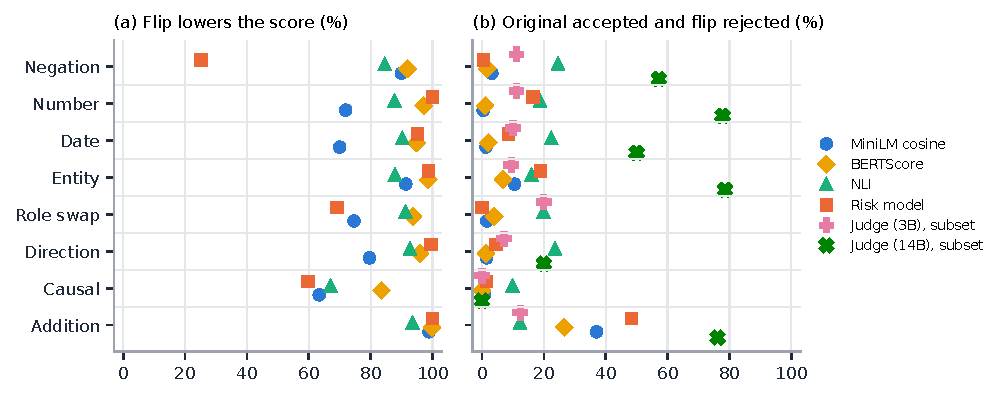
\includegraphics[width=\textwidth]{../figures/fig_cf_types.pdf}
\caption{Counterfactual sensitivity by perturbation type. (a) Share of flips that lower the score. (b) Paired detection: the unedited answer is accepted and the flip is rejected at the threshold fitted on natural calibration data.}
\label{fig:cftypes}
\end{figure*}

\paragraph{Scores move, decisions do not.} A single-fact flip lowers MiniLM's mean-max cosine in \CfCosDrop\% of pairs (Table~\ref{tab:cfdrop}), and the share is at least as high for BGE-small, BERTScore and NLI. Score-drop rates therefore make every method look sensitive. Decisions tell a different story (Figure~\ref{fig:cftypes}b, Table~\ref{tab:cfdetect}): with thresholds fitted on natural data, cosine accepts the unedited answer and rejects the flip in only \CfCosDetect\% \CfCosDetectCi\ of pairs. It rejects \CfCosFlipRej\% of flipped answers, but it accepts only \CfCosOrigAcc\% of the unedited faithful answers in the first place, so most rejections of flips are rejections the original would have received too. It accepts paraphrases about as often as the originals (\CfCosParaAcc\% vs.\ \CfCosParaOrigAcc\%), and among paraphrases whose original was accepted it rejects only \CfCosParaFalseRej\%. The descriptive half of H1 therefore holds: cosine is stable under rewording and rarely turns an accepted answer into a rejected one when a fact is changed. Paired detection is \CfNliDetect\% for NLI, \CfRiskDetect\% for the full risk model and \CfRiskChkDetect\% for the cosine-plus-checks variant; NLI exceeds cosine by \HoneNliMinusCos\ points \HoneNliMinusCosCi\ (Holm-adjusted $p\HoneNliHolm$).

The preregistered judge contrast of H1 uses the small judge (\CfJSmallN\ pairs, \CfJSmallBases\ bases; Table~\ref{tab:cfjudge}). It rejects \CfJSmallFlipRej\% of flips but accepts only \CfJSmallOrigAcc\% of originals, so its paired detection (\CfJSmallDetect\%) does not differ from cosine's (\HoneJudgeMinusCos\ points \HoneJudgeMinusCosCi, Holm-adjusted $p\HoneJudgeHolm$): H1 holds against NLI but not against the small judge. In an exploratory run (\CfJStrongN\ pairs, \CfJStrongBases\ bases, mostly additions, entities and negations), the 14B judge detects \CfJStrongDetect\% \CfJStrongDetectCi, \CfJStrongMinusCos\ points more than cosine \CfJStrongMinusCosCi\ and \CfJStrongMinusNli\ more than NLI \CfJStrongMinusNliCi\ on the same pairs---the only evaluator whose decisions track single-fact edits.

\paragraph{Inversion isolates sensitivity to the fact.} The paired detection rate is bounded by how often the original is accepted, and the score-drop rate rewards any change of wording. The inversion rate avoids both: holding the sentence, the evidence and the rest of the answer fixed, it asks whether the factual error scores at least as high as a harmless paraphrase. Here the methods separate sharply. NLI inverts in \CfNliInv\% \CfNliInvCi\ of triplets, MiniLM and BGE-small cosine in \CfCosInv\% and \CfBgeInv\%, BERTScore in \CfBertInv\%, the full risk model in \CfRiskInv\% and token precision in \CfTokPrecInv\%; MiniLM min-max cosine, which is driven by the least-supported sentence, inverts in most triplets. For a cosine score a paraphrase and a factual error are close to interchangeable, and the distributions of their score changes overlap almost completely (Figure~\ref{fig:locus}a).

\begin{figure*}[t]
\centering
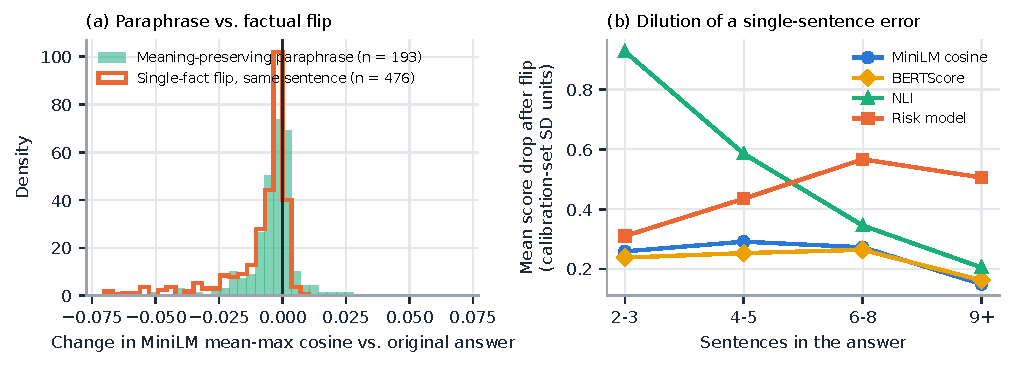
\includegraphics[width=\textwidth]{../figures/fig_locus.pdf}
\caption{(a) Change in MiniLM mean-max cosine caused by a meaning-preserving paraphrase and by a single-fact flip of the same sentence. (b) Mean score drop caused by a flip, in calibration-set standard deviations, by the number of sentences in the answer.}
\label{fig:locus}
\end{figure*}

\paragraph{Error types differ (H2).} Detection depends on the type of edit for every evaluator (within-base permutation test, $p\HtwoCosPerm$ for each; Cram\'er's $V$ from \CfNliCramerV\ for NLI to \CfRiskCramerV\ for the risk model). Unsupported additions are the only edit that cosine detects with any regularity (\CfCosDetectAddition\% paired detection); for numbers, dates, causal connectives and direction words its paired detection is \CfCosDetectNumber\%, \CfCosDetectDate\%, \CfCosDetectCausal\% and \CfCosDetectDirection\%. NLI is the most uniform across types (\CfNliDetectCausal\% to \CfNliDetectNegation\%) and the only method with substantial negation detection (\CfNliDetectNegation\%, against \CfCosDetectNegation\% for MiniLM). The explicit number and entity checks raise the risk model's detection of number and entity flips (\CfRiskDetectNumber\% and \CfRiskDetectEntity\%) but not of negation: a negation flip lowers the full model's support score in only \CfRiskDropNegation\% of pairs. Its strongest inputs barely react to negation---token precision falls for only \CfTokPrecDropNegation\% of negation flips, since words such as ``not'' usually occur somewhere in the evidence---and the weight it learned on the negation-mismatch feature is small and negative (Table~\ref{tab:coef}). A feature-based detector inherits the error distribution of its training labels.

\paragraph{Dilution.} Because cosine and NLI average over answer sentences, a fixed one-sentence error matters less in a longer answer (Figure~\ref{fig:locus}b). For NLI the mean drop falls from \CfNliDilFirst\ to \CfNliDilLast\ calibration standard deviations between the shortest and the longest answers; cosine's drop is small at every length (\CfCosDilFirst\ to \CfCosDilLast). The risk model, which includes per-sentence minima and counts of unsupported numbers and entities, does not dilute in the same way.

\subsection{Threshold transfer (RQ3)}
\label{sec:res-transfer}

\begin{figure*}[t]
\centering
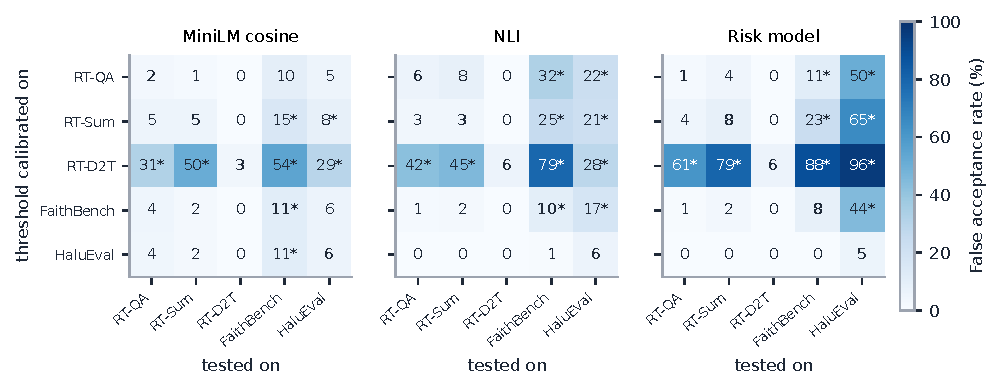
\includegraphics[width=\textwidth]{../figures/fig_transfer.pdf}
\caption{False-acceptance rate (\%) on the test split of the column domain when the threshold is calibrated to $\mathrm{FAR}\le5\%$ on the row domain. Bold: in-domain cells. *: the lower 95\% bound exceeds 5\%.}
\label{fig:transfer}
\end{figure*}

A threshold calibrated to $\mathrm{FAR}\le5\%$ mostly holds in its own domain: only \TrCosDiagExceed\ of the five diagonal cosine cells, FaithBench, has a lower confidence bound above 5\% (FAR \TrCosDiagMax\%), and the other in-domain cells stay close to the budget (Figure~\ref{fig:transfer}). The other evaluators behave similarly in-domain (one or two exceeding cells each, all below 14\%), except the full risk model, which has none. Across domains it does not. For MiniLM cosine \HthreeExceed\ of \HthreeCells\ off-diagonal cells exceed 5\% with the lower bound above 5\%, up to \TrCosOffMax\%, which supports H3 by the preregistered criterion (Bonferroni-adjusted bootstrap $p=\HthreePBonf$). The failure is not specific to cosine: the corresponding counts are \TrBgeOffExceed\ for BGE-small, \TrBertOffExceed\ for BERTScore, \TrNliOffExceed\ for NLI and \TrRiskOffExceed\ for the risk model, whose worst cell reaches \TrRiskOffMax\%. Thresholds learned on RT-D2T, where two thirds of answers are unsupported and support scores are low throughout, are the most permissive elsewhere; thresholds learned on FaithBench and HaluEval-QA are conservative on RAGTruth. Within RAGTruth, a threshold calibrated on long answers and applied to short ones raises cosine FAR to \ShLenCosLongToShort\% and the risk model's to \ShLenRiskLongToShort\%, whereas changing the generator family moves FAR by a few points only (Table~\ref{tab:shift}). Calibrated probabilities do not transfer either: the risk model's expected calibration error is \CalQaEce\ on RT-QA but \CalFbEce\ on FaithBench and \CalHaluEce\ on HaluEval-QA.

\subsection{Selective evaluation (RQ4)}
\label{sec:res-cascade}

\paragraph{Cheap stage.} On the full RAGTruth test set at $\alpha=0.05$ and $\beta=0.10$ (Table~\ref{tab:cheapstage}), the cosine gate resolves \CsCosFiveCov\% \CsCosFiveCovCi\ of answers without a judge, with a cheap-stage FAR of \CsCosFiveFar\%. The full risk model resolves \CsRiskFiveCov\% \CsRiskFiveCovCi\ at a cheap-stage FAR of \CsRiskFiveFar\%, \HfourRiskDiff\ points more than cosine \HfourRiskDiffCi\ (Holm-adjusted $p\HfourHolm$); NLI and BGE-small resolve \HfourNliDiff\ and \HfourBgeDiff\ points more than MiniLM. The cosine-plus-checks variant does not resolve more than cosine (\HfourRiskChkDiff\ points, \HfourRiskChkDiffCi). Within domain the calibration-time FAR budget is approximately met by every gate; on FaithBench, with thresholds carried over from RT-Sum, the cheap-stage FAR rises to \FbOodCosFar\% for cosine and \FbOodRiskFar\% for the risk model.

\begin{table*}[t]
\centering\small
\resizebox{\textwidth}{!}{\begin{tabular}{llrlrrlr}
\toprule
Policy & Gate & Judged\,\% & BAcc [95\% CI] & FAR\,\% & FRR\,\% & $\Delta$BAcc vs.\ always-judge & Random \\
\midrule
Always judge & -- & 100.0 & .566 [.543, .592] & 1.6 & 85.2 & -- & -- \\
\midrule
Never judge & Token precision & 0.0 & .569 [.516, .627] & 48.1 & 38.1 & .004 [-.051, .063] & -- \\
Never judge & MiniLM cosine (mean-max) & 0.0 & .625 [.581, .667] & 33.3 & 41.8 & .059 [.015, .100] & -- \\
Never judge & BGE-small cosine (mean-max) & 0.0 & .559 [.513, .603] & 41.0 & 47.2 & -.006 [-.057, .041] & -- \\
Never judge & BERTScore & 0.0 & .567 [.514, .617] & 49.2 & 37.5 & .001 [-.055, .056] & -- \\
Never judge & NLI (SummaC-ZS style) & 0.0 & .585 [.538, .631] & 34.4 & 48.6 & .019 [-.030, .068] & -- \\
Never judge & Risk model: full & 0.0 & .634 [.583, .681] & 36.1 & 37.2 & .068 [.017, .117] & -- \\
\midrule
Gate, $\alpha=0.05$ & MiniLM cosine (mean-max) & 75.9 & .581 [.550, .613] & 7.1 & 76.7 & .015 [-.009, .041] & .579 \\
Gate, $\alpha=0.05$ & NLI (SummaC-ZS style) & 73.3 & .583 [.551, .616] & 10.9 & 72.4 & .017 [-.009, .045] & .571 \\
Gate, $\alpha=0.05$ & Risk model: cosine + checks & 77.9 & .595 [.566, .625] & 4.4 & 76.7 & .029 [.007, .051] & .596 \\
Gate, $\alpha=0.05$ & Risk model: full & 64.5 & .635 [.601, .671] & 7.7 & 65.3 & .069 [.039, .101] & .589 \\
\midrule
Gate, $\alpha=0.1$ & MiniLM cosine (mean-max) & 67.1 & .594 [.559, .627] & 13.1 & 68.2 & .028 [-.004, .060] & .587 \\
Gate, $\alpha=0.1$ & NLI (SummaC-ZS style) & 63.4 & .608 [.573, .643] & 16.4 & 61.9 & .043 [.013, .072] & .572 \\
Gate, $\alpha=0.1$ & Risk model: cosine + checks & 67.9 & .631 [.599, .665] & 8.7 & 65.1 & .065 [.036, .094] & .610 \\
Gate, $\alpha=0.1$ & Risk model: full & 58.3 & .664 [.629, .699] & 8.7 & 58.5 & .098 [.066, .132] & .595 \\
\midrule
Gate, $\alpha=0.2$ & MiniLM cosine (mean-max) & 53.8 & .625 [.585, .663] & 20.2 & 54.8 & .059 [.020, .096] & .593 \\
Gate, $\alpha=0.2$ & NLI (SummaC-ZS style) & 49.2 & .619 [.577, .659] & 27.3 & 48.9 & .053 [.014, .093] & .576 \\
Gate, $\alpha=0.2$ & Risk model: cosine + checks & 53.1 & .643 [.605, .681] & 19.1 & 52.3 & .077 [.040, .113] & .631 \\
Gate, $\alpha=0.2$ & Risk model: full & 41.1 & .678 [.636, .720] & 21.9 & 42.6 & .112 [.070, .153] & .607 \\
\bottomrule
\end{tabular}
}
\caption{System results on the RAGTruth and FaithBench judged subset ($n=\SysSmallN$) with the small judge. ``Judged'' is the share escalated; ``Random'' is the mean balanced accuracy when the same number of randomly chosen examples is escalated and the rest decided by the gate's $\tau^\mathrm{bal}$.}
\label{tab:cascadesmall}
\end{table*}

\paragraph{System.} With the small judge (Table~\ref{tab:cascadesmall}), always judging gives a balanced accuracy of only \SysSmallJudgeBacc\ on the judged subset, because the judge rejects most faithful answers. Every cascade is at least as good, and the risk-gated cascade at $\alpha=0.05$ is \SysSmallRiskFiveDiff\ \SysSmallRiskFiveDiffCi\ better while sending \SysSmallRiskFiveEsc\% of examples to the judge; random escalation of the same share gives \SysSmallRiskFiveRand. The second condition of H4 (no more than two points below always-judge) is therefore met, but trivially, because the reference point is weak; the escalation curves (Figure~\ref{fig:escalation}) show that with this judge the best policy escalates only a small share of examples, and that escalating the smallest-margin examples first beats random escalation clearly for the risk model, slightly for NLI and not at all for cosine.

With the 14B judge on its \SysStrongN\ RAGTruth answers (Table~\ref{tab:cascadestrong}), the ordering reverses. Judging everything gives \SysStrongJudgeBacc\ \SysStrongJudgeBaccCi, and every cheap method alone is worse (cosine \SysStrongNeverCosDiff\ \SysStrongNeverCosDiffCi, full risk model \SysStrongNeverRiskDiff\ \SysStrongNeverRiskDiffCi). The cascades now trade accuracy for judge calls. The cosine gate at $\alpha=0.05$ skips \SysStrongCosFiveSaved\% of judge calls at \SysStrongCosFiveDiff\ \SysStrongCosFiveDiffCi; the risk gate skips \SysStrongRiskFiveSaved\% at \SysStrongRiskFiveDiff\ \SysStrongRiskFiveDiffCi; the cosine-plus-checks gate skips \SysStrongRiskChkFiveSaved\% at \SysStrongRiskChkFiveDiff\ \SysStrongRiskChkFiveDiffCi. The intervals include both no loss and losses well beyond the two-point margin of H4, so on this subset the accuracy condition of H4 can be neither confirmed nor rejected for the stronger judge. Targeted escalation still beats random escalation of the same share for the risk gate (\SysStrongRiskFiveBacc\ vs.\ \SysStrongRiskFiveRand).

\begin{figure*}[t]
\centering
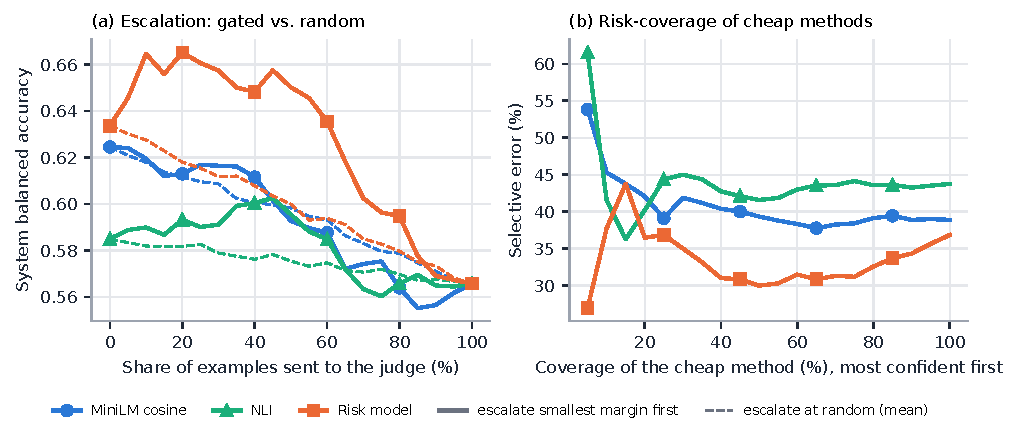
\includegraphics[width=\textwidth]{../figures/fig_escalation.pdf}
\caption{(a) System balanced accuracy on the small-judge subset as a function of the share escalated, escalating the smallest-margin examples first (solid) or at random (dashed, mean over draws). (b) Risk--coverage curves of the cheap methods alone.}
\label{fig:escalation}
\end{figure*}

\paragraph{Correctness.} On the full EVOUNA-NQ test set the reference-mode risk model resolves \EvCsRiskCov\% of answers at a cheap-stage FAR of \EvCsRiskFar\%. On the 600 judged answers it escalates \EvCsRiskEsc\% to the small judge, and the system reaches a balanced accuracy of \EvCsRiskSysBacc; the cosine-gated system escalates \EvCsCosEsc\% and reaches \EvCsCosSysBacc.

\subsection{Cost (RQ5)}
\label{sec:cost}

\begin{table*}[t]
\centering\small
\resizebox{\textwidth}{!}{\begin{tabular}{lrrrrrrr}
\toprule
Method & Median ms & p95 ms & Wall s / 1k & CPU s / 1k & Cold start s & Prompt tok. & Out tok. \\
\midrule
Lexical features + checks & 1.4 & 2.8 & 1.5 & 2 & 0.0 & -- & -- \\
MiniLM cosine & 321 & 1,083 & 433 & 2,574 & 6.4 & -- & -- \\
\quad evidence embeddings cached & 42.9 & 83.2 & 49.1 & 292 & 6.4 & -- & -- \\
BGE-small cosine & 631 & 2,046 & 831 & 4,934 & 1.8 & -- & -- \\
\quad evidence embeddings cached & 85.1 & 163 & 95.6 & 562 & 1.8 & -- & -- \\
Risk model: full & 414 & 1,164 & 513 & 3,046 & 6.4 & -- & -- \\
\midrule
BERTScore (roberta-base) & 1,005 & 1,945 & 1,039 & 6,122 & 1.7 & -- & -- \\
NLI (DeBERTa-v3-base) & 2,302 & 5,865 & 2,900 & 15,206 & 9.7 & -- & -- \\
\midrule
Judge (3B), new source & 10,292 & 23,181 & 11,791 & -- & 4.4 & 861 & 9.0 \\
\quad same source (prefix cached) & 4,711 & 5,955 & 4,736 & -- & 4.4 & 839 & 9.0 \\
\midrule
Judge (14B), new source & 38,475 & 95,366 & 46,463 & -- & 15.7 & 867 & 10.1 \\
\quad same source (prefix cached) & 13,547 & 19,472 & 13,953 & -- & 15.7 & 846 & 9.4 \\
\bottomrule
\end{tabular}
}
\caption{Measured cost on one CPU-only laptop (\HwCores\ logical cores, \HwRam\,GB RAM, \HwThreads\ PyTorch threads, no GPU), on a fixed sample of \CostSampleN\ RAGTruth answers (mean \CostAnsWords\ answer words, \CostEvWords\ evidence words), single process, no other job running. Wall and CPU seconds per 1{,}000 evaluations exclude cold start, which is reported separately. Judge rows: 30 calls each; ``prefix cached'' is a second answer for the same source, for which the server reuses the cached evidence prefix. No paid API was used, so no monetary cost is reported.}
\label{tab:cost}
\end{table*}

\begin{figure*}[t]
\centering
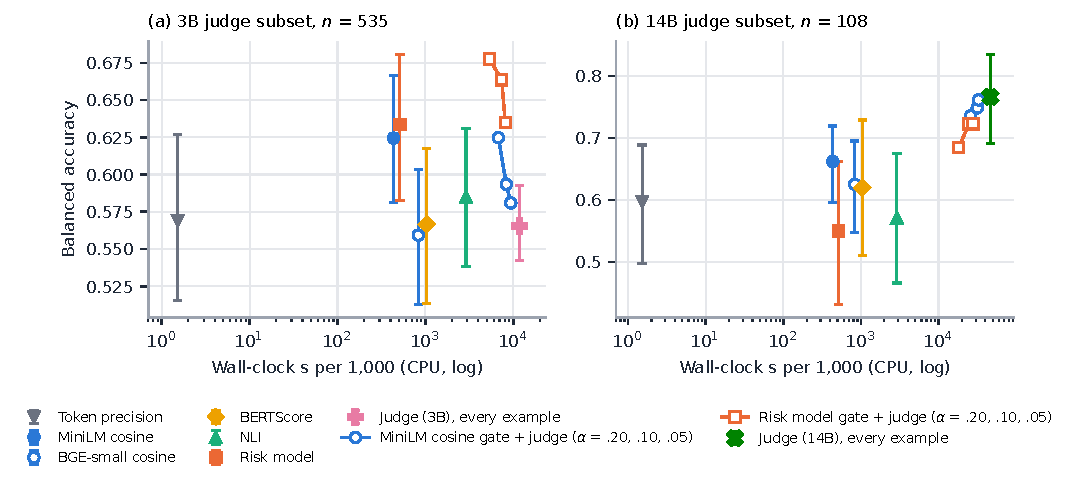
\includegraphics[width=\textwidth]{../figures/fig_pareto.pdf}
\caption{Balanced accuracy against measured wall-clock cost per 1{,}000 evaluations on the two judged subsets. Cascade cost is the cheap-stage cost for every example plus the judge cost for the escalated share. Error bars: 95\% cluster-bootstrap intervals. The panels use different examples and are not directly comparable.}
\label{fig:pareto}
\end{figure*}

Table~\ref{tab:cost} reports measured cost. Lexical features with the number and entity checks take \CostLexicalAndChecksWall\,s per 1{,}000 answers. MiniLM cosine takes \CostMinilmCosineWall\,s including evidence encoding and \CostMinilmCosineEvidenceCachedWall\,s when evidence embeddings are cached; the full risk model, which needs MiniLM embeddings, takes \CostRiskFullWall\,s. Relative to MiniLM cosine with evidence encoding, BERTScore costs \CostBertscoreRatio$\times$, NLI \CostNliRatio$\times$, the 3B judge \CostJudgeSmallRatio$\times$ (\CostJudgeSmallPrefixCachedRatio$\times$ when the evidence prefix is cached) and the 14B judge \CostJudgeStrongRatio$\times$ (\CostJudgeStrongPrefixCachedRatio$\times$). Judge cost is dominated by reading the prompt (about \CostJudgeSmallPtok\ tokens, processed at \CostJudgeSmallTokPerS\ tokens/s by the 3B and \CostJudgeStrongTokPerS\ tokens/s by the 14B model), which is why prefix caching helps so much when several answers share one source.

Figure~\ref{fig:pareto} combines cost with accuracy. With the 3B judge, the risk gate is better and cheaper than judging everything at every $\alpha$; at $\alpha=0.20$ it reaches \SysSmallRiskTwentyBacc\ while judging \SysSmallRiskTwentyEsc\% of examples. With the 14B judge, every cheap method alone is far below the judge, and the gates save between a quarter and two fifths of judge time at an accuracy cost that this subset cannot pin down. These cost figures are specific to one CPU laptop; we did not measure GPU inference, where the ratios between methods may differ.
